\documentclass{article}

\usepackage{listings}
\usepackage{graphicx}
\usepackage{float}
\usepackage{array}
\usepackage{amssymb}
\usepackage{amsmath}
\usepackage{booktabs}
\usepackage{listings}
\usepackage{xcolor}
\usepackage{minted}
\usepackage[utf8]{inputenc}
\usepackage{caption}

\captionsetup[figure]{name=Figura}

\lstset{
  language=Python,        % Lenguaje del código
  basicstyle=\ttfamily,   % Fuente tipo máquina de escribir
  keywordstyle=\color{blue}, % Color para palabras clave
  commentstyle=\color{gray}, % Color para comentarios
  stringstyle=\color{red},   % Color para strings
  frame=single,          % Marco alrededor del código
  numbers=left,          % Numeración de líneas
  numberstyle=\tiny,     % Tamaño de los números de línea
  breaklines=true,       % Cortar líneas largas
  tabsize=4
}

\begin{document}
  \begin{titlepage}
    \centering
    \vspace*{2cm}
    
    \Huge
    \textbf{Informe Final SCN}
    
    \vspace{1.5cm}
    
    \Large
    Jhorman Gomez{\textsuperscript{1}}
    Nicolas Salazar{\textsuperscript{2}}
    
    \vspace{0.5cm}
    
    \large

    2326867{\textsuperscript{1}}
    2328060{\textsuperscript{2}}
  
    
    \vspace{0.5cm}
    
    \Large
    Universidad del Valle
    
    \vspace{0.5cm}
    
    \large
    Facultad de Ingeniería
    
    \vspace{0.5cm}
    
    \large
    Escuela de Ingeniería de Sistemas y Computación
    
    \vspace{0.5cm}
    
    \large
    Santiago de Cali, Mayo de 2025
    
  \end{titlepage}

  \section*{Abstract}
  \paragraph{}
  Este trabajo presenta una simulación numérica de la velocidad de un fluido incompresible usando la discretización de las ecuaciones de Navier-Stokes. El problema se modeló sobre una malla rectangular, donde la velocidad en cada punto se calcula como un promedio de las velocidades en las celdas adyacentes, ajustado por un término no lineal. Para resolver el sistema asociado al problema, se empleó el método de Newton-Raphson, mientras que para el cálculo del vector de corrección de Newton-Raphson se exploraron métodos iterativos como Richardson, Jacobi, Gauss-Seidel, y métodos de Krylov como Gradiente Conjugado y Gradiente Descendiente.

  \section*{Introducción}
  \paragraph{}
  El presente trabajo se enmarca en el campo de la dinámica de fluidos, específicamente en la simulación numérica de la vorticidad de un fluido incompresible a través de la discretización de las ecuaciones de Navier-Stokes. El objetivo principal de este estudio es modelar numéricamente el comportamiento de la vorticidad en un medio continuo, explorando y aplicando distintos métodos numéricos para su resolución.

  \paragraph{}
  El objetivo específico planteado es comparar distintos métodos númericos para la solución de sistemas lineales, con el propósito de identificar cuáles son aplicables a nuestro problema y determinar aquel que presenta un mejor desempeño en términos del número de iteraciones requeridas para alcanzar la convergencia. Los métodos evaluados incluyen Richardson, Jacobi, Gauss-Seidel, Gradiente Descendiente y Gradiente Conjugado.
  
  \paragraph{}
  A lo largo del desarrollo del proyecto, se concluyó que el método de Gauss-Seidel presenta un mejor comportamiento para este problema en particular, logrando una convergencia más rápida con un menor número de iteraciones. Adicionalmente, se identificó que los métodos de Krylov no pueden aplicarse en este contexto, debido a que la matriz generada en el sistema lineal asociado al método de Newton-Raphson no es simétrica, siendo este un requisito para su implementación.

  \section*{Metodología}

  El proceso de desarrollo del proyecto siguió un ciclo de pequeños avances conforme se desarrollaban los contenidos del curso. Este ciclo puede describirse de la siguiente manera:

  \begin{enumerate}
      \item \textbf{Adquisición de conocimiento teórico:} 
      El proceso inició con la revisión de conceptos teóricos durante las clases. Entre estos conceptos se incluyen temas como diferencias finistas, Newton-Raphson para solución de sistemas no lineales, métodos iterativos y de Krylov para solución de sistemas lineales, entre otros.
      
      \item \textbf{Aplicación al proyecto:}  
      Tras comprender los conceptos teóricos, se procedió a su aplicación en el proyecto:
      
      \begin{itemize}
          \item \textbf{Discretización de las ecuaciones de Navier-Stokes:}  
          Una vez entendido el método de diferencias finitas, se discretizaron las ecuaciones en el dominio del problema, eligiendo parámetros iniciales como el tamaño de malla y el step ($h$) adecuado para las simulaciones.  

          \item \textbf{Implementación de Newton-Raphson:}  
          Con el método de Newton-Raphson se calculó la solución aproximada del sistema de ecuaciones no lineales, permitiendo realizar la primera simulación del proyecto.  

          \item \textbf{Análisis e implementación de métodos iterativos y de Krylov:}  
          Al avanzar en los temas, se exploraron diferentes métodos iterativos (Richardson, Jacobi, Gauss-Seidel) y métodos de Krylov (Gradiente Descendiente y Gradiente Conjugado) para calcular el vector de corrección en el método de Newton-Raphson.
      \end{itemize}
      
      \item \textbf{Implementaciones:}  
      Cada avance fue implementado en Python. Las simulaciones realizadas fueron guardadas para su posterior presentación en clase.
      
      \item \textbf{Retroalimentación constante:}  
      Para cada avance se realizó una breve presentación frente a la profesora, donde se expusieron los avances y se recibió retroalimentación. Esto permitió corregir errores y reafirmar conceptos antes de seguir con el siguiente ciclo. 
  \end{enumerate}

  \section*{Desarrollo del Proyecto}

  \subsection*{Primer Avance}
  \paragraph{}
  Durante el primer avance se tuvo como objetivvo definir parámetros como la dimensión, el step $h$, las ecuaciones y condiciones de frontera de la malla.

  \paragraph{}
  Para los parámetros iniciales decidimos que usariamos los siguientes valores:

  \[Nx=60, \ Ny=20, \ h=1\]

  $N_x$ y $N_y$ representando el número de columnas y filas respectivamente, generando así un sistema de $1200$ ecuaciones, una cantidad que creemos manejable y por ende el por qué de estas dimensiones.

  \begin{figure}[h!]
    \centering
    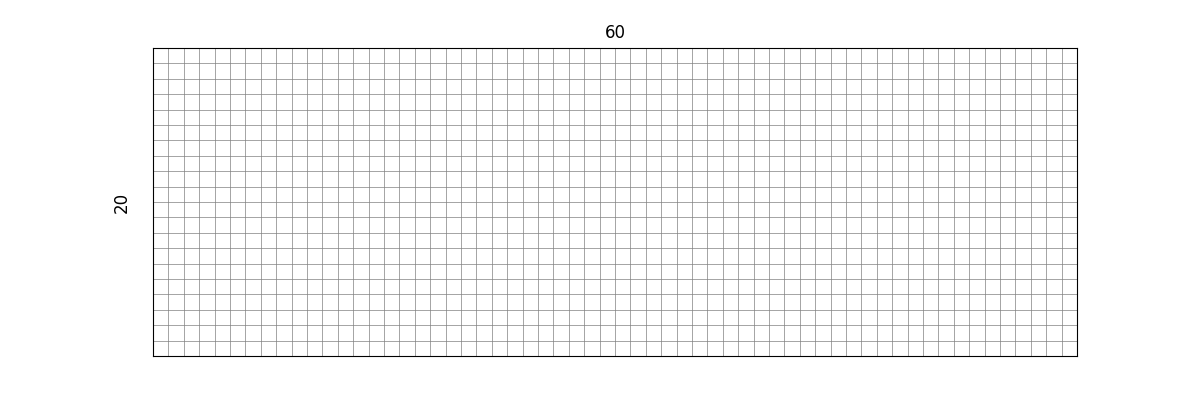
\includegraphics[width=1\textwidth]{PrimerMalla.png}
    \caption{Primer Malla}
  \end{figure}

  \paragraph{}
  Posteriormente definimos nuestras condiciones de frontera sobre la malla:

  \

  Borde superior
  \[V_x = 0, \, v_y = 0 \quad i = 0, \quad 0 \leq j \leq 59\]

  Borde inferior
  \[v_x = 0, \, v_y = 0 \quad i = 19, \quad 0 \leq j \leq 59\]

  Borde izquierdo
  \[v_x = 1, \, v_y = 0 \quad j = 0, \quad 0 < i < 19\]

  Borde derecho
  \[v_x = 1, \, v_y = 0 \quad j = 59, \quad 0 < i < 19\]

  \paragraph{}
  Por último, partiendo de la siguiente ecuación:

  \[r=\frac{1}{4}[v_{i+1,j}^x+v_{i-1,j}^x+v_{i,j+1}^x+v_{i,j-1}^x]+N-v_{i,j}^x\]
  
  consideraremos que este residuo $r$ es $0$ obteniendo:
  \[v_{i,j}^x=\frac{1}{4}[v_{i+1,j}^x+v_{i-1,j}^x+v_{i,j+1}^x+v_{i,j-1}^x]+N\]
  \[N=-\frac{h}{8}v_{i,j}^x(v_{i+1,j}^x-v_{i-1,j}^x)-\frac{h}{8}v_{i,j}^y(v_{i,j+1}^x-v_{i,j-1}^x)\]

  \paragraph{}
  la velocidad en una celda cualquiera será dada por un promedio de las velocidades de las celdas adyacentes más un factor no lineal.

  \paragraph{}
  Teniendo en cuenta las condiciones de frontera mencionadas, los parámetros iniciales definidos y la ecuación para la velocidad de cada celda, la malla estará conformada por bordes con valores constantes y celdas internas que, dependiendo de su posición en la malla interior (centro, borde o esquina), tendrán una ecuación diferente:

  \

  Borde superior interno
  \[v^{x}_{1,j} = \frac{1}{4}[v^x_{2,j} + v^x_{1,j+1} + v^x_{1,j-1} - \frac{h}{2}v^{x}_{1,j}(v^x_{2,j})- \frac{h}{2}v^{y}_{1,j}(v^x_{1,j+1}-v^x_{1,j-1})]\]
  \[1<j<58\]

  Borde inferior interno
  \[v^{x}_{18,j} = \frac{1}{4}[v^x_{17,j} + v^x_{18,j+1} + v^x_{18,j-1} - \frac{h}{2}v^{x}_{18,j}(-v^{x}_{17,j})- \frac{h}{2}v^{y}_{18,j}(v^x_{18,j+1}-v^x_{18,j-1})]\]
  \[1<j<58\]

  Borde izquierdo interno
  \[v_{i,1}^x=\frac{1}{4}[v_{i+1,1}^x+v_{i-1,1}^x+v_{i,2}^x+1 - \frac{h}{2}v^{x}_{i,j}(v^{x}_{i+1,j}-v^{x}_{i-1,j})- \frac{h}{2}v^{y}_{i,j}(v^x_{i,j+1}-1)]\]
  \[1<i<18\]

  Borde derecho interno
  \[v_{i,58}^x=\frac{1}{4}[v_{i+1,58}^x+v_{i-1,58}^x+v_{i,57}-\frac{1}{2}v_{i,58}^x(v_{i+1,j}^x-v_{i-1,j}^x)-\frac{1}{2}v_{i,58}^y(-v_{i,57}^x)]\]
  \[1<i<18\]

  Esquina superior izquierda
  \[v_{1,1}^x=\frac{1}{4}[v_{2,1}^x+v_{1,2}^x+1-\frac{1}{2}v_{1,1}^x(v_{2,1}^x)-\frac{1}{2}v_{1,1}^y(v_{1,2}^x-1)]\]

  Esquina superior derecha
  \[v_{1,58}^x=\frac{1}{4}[v_{2,1}^x+v_{1,57}^x-\frac{1}{2}v_{1,58}^x(v_{2,1}^x)-\frac{1}{2}v_{1,58}^y(-v_{1,57}^x)]\]

  Esquina inferior izquierda
  \[v_{18,1}^x=\frac{1}{4}[v_{17,1}^x+v_{18,2}^x+1-\frac{1}{2}v_{18,1}^x(-v_{17,1}^x)-\frac{1}{2}v_{18,1}^y(v_{18,2}^x-1)]\]

  Esquina inferior derecha
  \[v_{18,58}^x=\frac{1}{4}[v_{17,58}^x+v_{18,57}^x-\frac{1}{2}v_{18,58}^x(-v_{17,58}^x)-\frac{1}{2}v_{18,58}^y(-v_{18,57}^x)]\]

  Centro
  \[v_{i,j}^x=\frac{1}{4}[v_{i+1,j}^x+v_{i-1,j}^x+v_{i,j+1}^x+v_{i,j-1}^x]+N\]
  \[N=-\frac{h}{8}v_{i,j}^x(v_{i+1,j}^x-v_{i-1,j}^x)-\frac{h}{8}v_{i,j}^y(v_{i,j+1}^x-v_{i,j-1}^x)\]
  \[2<i<18, \ 2<j<58\]

  \subsection*{Segundo Avance}
  \paragraph{}
  Para el segundo avance, el objetivo fue aplicar el método de \textbf{Newton-Raphson} para solucionar el sistema de ecuaciones asociado al problema. Dicho sistema está conformado por ecuaciones de la forma:

  \[
  F_{i,j} = v_{(i,j)}^x - \frac{1}{4} \left[v_{(i+1,j)}^x + v_{(i-1,j)}^x + v_{(i,j+1)}^x + v_{(i,j-1)}^x \right] + N
  \]

  donde \(N\) representa el término no lineal que depende de las diferencias de velocidades adyacentes y se define como:

  \[
  N = \frac{h}{8}v_{(i,j)}^x \left(v_{(i+1,j)}^x - v_{(i-1,j)}^x \right) + \frac{h}{8}v_{(i,j)}^y \left(v_{(i,j+1)}^x - v_{(i,j-1)}^x \right)
  \]

  el sistema de ecuaciones generado tiene un total de \((N_x - 2) \cdot (N_y - 2)\) ecuaciones, es decir, \(1044\) ecuaciones en nuestro caso, considerando las condiciones de frontera.

  \paragraph{}
  El método de \textbf{Newton-Raphson} para sistemas de ecuaciones de varias variables se expresa mediante la siguiente ecuación iterativa \cite{kincaid1}:

  \[
  \vec{x}^{(k+1)} = \vec{x}^{(k)} + H
  \]

  donde:
  \begin{itemize}
    \item \(\vec{x}\) es el vector de incógnitas que representa las velocidades en cada celda interna de la malla.
    \item \(H\) es el incremento calculado en cada iteración para aproximarnos a la solución.
  \end{itemize}

  \paragraph{}
  El incremento \(H\) se obtiene resolviendo el sistema lineal siguiente:

  \[
  J(\vec{x}^{(k)}) H = -F(\vec{x}^{(k)})
  \]

  donde:
  \begin{itemize}
    \item \(J(\vec{x})\) es la matriz jacobiana del sistema evaluada en el punto actual. Esta se forma a partir de las derivadas parciales de cada ecuación \(F_{i,j}\) respecto a cada incógnita:
      
    \[
    J(\vec{x}) = 
    \begin{pmatrix} 
    \frac{\partial F_1}{\partial x_1} & \frac{\partial F_1}{\partial x_2} & \cdots & \frac{\partial F_1}{\partial x_n} \\ 
    \frac{\partial F_2}{\partial x_1} & \frac{\partial F_2}{\partial x_2} & \cdots & \frac{\partial F_2}{\partial x_n} \\ 
    \vdots & \vdots & \ddots & \vdots \\ 
    \frac{\partial F_n}{\partial x_1} & \frac{\partial F_n}{\partial x_2} & \cdots & \frac{\partial F_n}{\partial x_n}
    \end{pmatrix}
    \]

    \item \(F(\vec{x})\) es la matriz de ecuaciones evaluada en el punto actual.
  \end{itemize}

  \paragraph{}
  Teniendo en cuenta la teoría desarrollada previamente, procedemos al cálculo del \textbf{Jacobiano} de nuestra malla. Debido a la estructura de las ecuaciones, para cada una de ellas únicamente existen cinco derivadas parciales no nulas. Esto implica que el Jacobiano adopta una forma similar a una matriz diagonal acompañada por cuatro sub-diagonales.

  \paragraph{}
  Los cinco tipos de derivadas parciales no nulas corresponden a las contribuciones de las celdas adyacentes en las siguientes direcciones:
  \begin{itemize}
      \item Derivada con respecto a \(v_{(i+1, j)}^x\) — Celda inferior.
      \[-\frac{1}{4}+\frac{h}{8}v_{(i,j)}^x\]
      \item Derivada con respecto a \(v_{(i-1, j)}^x\) — Celda superior.
      \[-\frac{1}{4}-\frac{h}{8}v_{(i,j)}^x\]
      \item Derivada con respecto a \(v_{(i, j+1)}^y\) — Celda a la izquierda.
      \[-\frac{1}{4}-\frac{h}{8}v_{(i,j)}^y\]
      \item Derivada con respecto a \(v_{(i, j-1)}^y\) — Celda a la derecha.
      \[-\frac{1}{4}+\frac{h}{8}v_{(i,j)}^y\]
      \item Derivada con respecto a \(v_{(i, j)}^x\) — Celda actual (término diagonal).
      \[1+\frac{h}{8}(v_{(i+1,j)}^x-v_{(i-1,j)}^x)\]
  \end{itemize}

  obteniendo así:

  \begin{figure}[H]
    \centering
    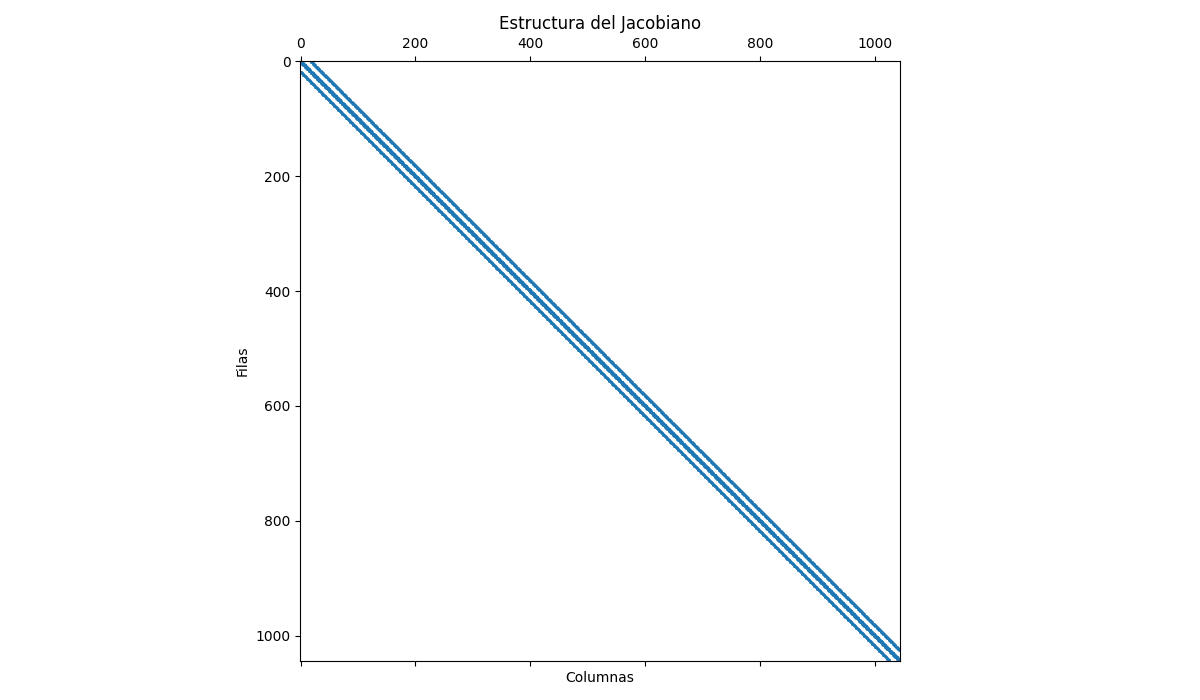
\includegraphics[width=1\textwidth]{Jacobiano.png}
    \caption{Jacobiano}
  \end{figure}

  \paragraph{}
  Una vez definido el Jacobiano y su estructura, el siguiente paso es implementar el método de Newton-Raphson para resolver el sistema de ecuaciones no lineales. Para ello, utilizaremos Python y la función \textbf{dgesv} de la librería \textbf{scipy}, la cual emplea factorización LU para resolver el sistema.

  \paragraph{}
  Es importante mencionar que el valor inicial seleccionado para el paso de malla, $h=1$, en el primer avance, fue modificado a $h=0.001$. Este cambio se realizó tras observar que las simulaciones con el valor anterior no arrojaban resultados consistentes con el comportamiento esperado. Además, el nuevo valor permite una convergencia más rápida del sistema. Teniendo en cuenta lo anterior, esta fue la solución obtenida:

  \begin{figure}[H]
    \centering
    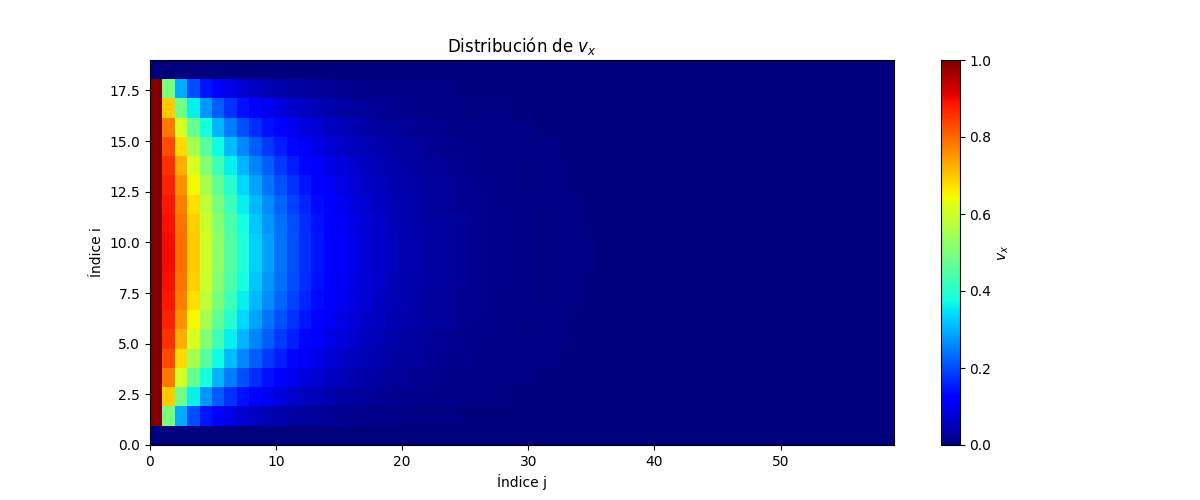
\includegraphics[width=1.2\textwidth]{GaussJordanSol.png}
    \caption{Primer Simulación}
  \end{figure}

  \subsection*{Tercer Avance}
  \paragraph{}
  En el tercer avance se tiene como objetivo la implementación de los métodos iterativos \textbf{Richardson}, \textbf{Jacobi} y \textbf{Gauss-Seidel}, y los métodos de Krylov \textbf{Grad. Descendiente} y \textbf{Grad. Conjugado}, para el cálculo del vector de correción $H$.

  \paragraph{}
  Antes de pasar al desarrollo de los objetivos de este avance es importante aclarar que hasta el momento las matrices $V_x$ y $V_y$ eran inicializacadas ambas con un valor constante igual para cada celda. Ahora, la forma en la que se inicializan es partiendo de unos valores iniciales $V_x^{0}$ y $V_y^{0}$ y un escalar $v$ dado, se dividen ambas matrices en $p$ particiones y se le asigna a cada perteneciente a una partición un valor dado por la fórmula:

  \[V_x^{(p)}=V_x^{(0)}\cdot v^{p+1}\]
  \[V_y^{(p)}=V_y^{(0)}\cdot v^{p+1}\]

  \paragraph{}
  En métodos iterativos como \textbf{Richardson}, \textbf{Jacobi} y \textbf{Gauss-Seidel} tenemos que la ecuación de iteración es:

  \[
  \vec{x}^{(k)}=(I-Q^{-1}A)\vec{x}^{(k-1)}+Q^{-1}b
  \]

  donde:
  \begin{itemize}
      \item $A$ en nuestro caso es el Jacobiano y $b$ es el vector de términos independientes obtenido de la matriz de ecuaciones.
      \item $Q$ varía dependiendo del método:
      \begin{itemize}
          \item Para Richardson, $Q$ es la matriz identidad.
          \item Para Jacobi, $Q$ es la matriz diagonal de $A$.
          \item Para Gauss-Seidel, $Q$ es la matriz triangular inferior de $A$.
      \end{itemize}
  \end{itemize}

  estos métodos convergen bajo los siguientes supuestos:
  \begin{itemize}
    \item Para los métodos de Gauss-Seidel y Jacobi, basta con que la matriz $A$ sea diagonal dominante \cite{kincaid2}.
    \item Para el método de Richardson, es necesario comprobar que $\|I-Q^{-1}A\| \leq 1$ para alguna norma dada \cite{kincaid2}.
  \end{itemize}

  recordemos que una matriz es diagonal dominante si:

  \[
  |a_{ii}| \geq \sum_{j \neq i}^{} |a_{ij}|
  \]

  procedemos entonces a verificar estos supuestos. Al ejecutar la siguiente función en python sobre nuestra matriz Jacobiana:

  \begin{figure}[H]
      \centering
      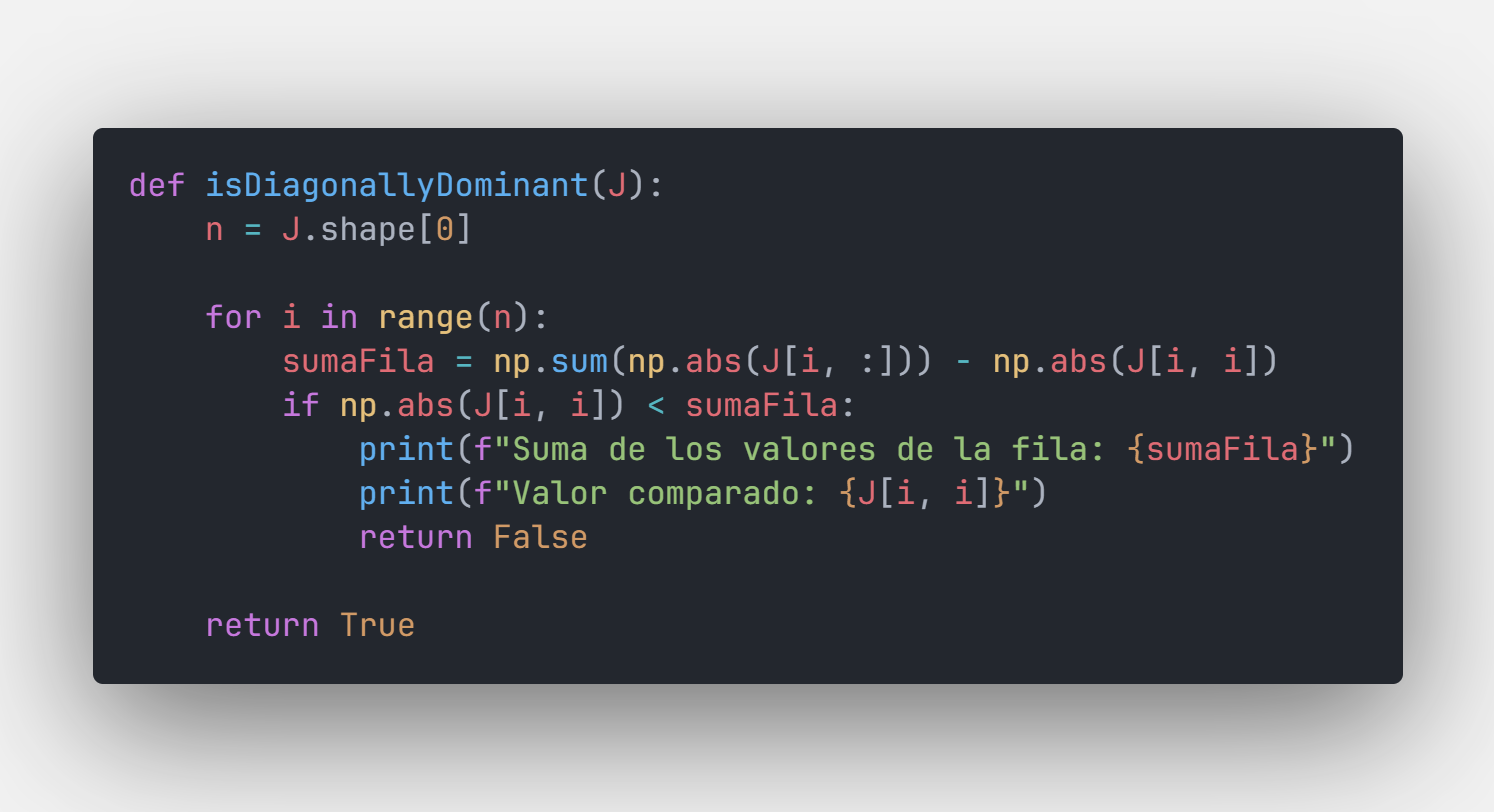
\includegraphics[width=1\textwidth]{DiagDom.png}
      \caption{Función \texttt{isDiagonallyDominant}}
  \end{figure}

  obtenemos que existen valores en la diagonal que son menores que la suma de los elementos restantes de la fila. Sin embargo, la diferencia es mínima, lo que puede atribuirse a pérdidas de precisión debido al redondeo de números. En consecuencia, consideraremos que la matriz es diagonalmente dominante, y por lo tanto, podemos aplicar los métodos de \textbf{Jacobi} y \textbf{Gauss-Seidel}.

  \paragraph{}
  En cuanto a \textbf{Richardson}, al realizar la prueba de convergencia obtenemos el siguiente valor para la norma infinito:

  \[
  \|I-Q^{-1}A\|_\infty = 1.0000415344381142
  \]

  este valor es ligeramente diferente de 1, pero la diferencia es pequeña, lo que nuevamente atribuimos a la pérdida de precisión por redondeo. Por lo tanto, consideraremos que se cumple el supuesto y, en consecuencia, podemos aplicar el método de Richardson.

  \paragraph{}
  Una vez cubiertos los métodos iterativos y sus respectivos supuestos, pasamos al análisis de los métodos de Krylov, en particular, el \textbf{Gradiente Descendiente} y el \textbf{Gradiente Conjugado}. Para aplicar estos métodos es necesario garantizar que la matriz $A$ cumple los siguientes requisitos:

  \begin{itemize}
      \item Es \textbf{simétrica}.
      \item Es \textbf{positiva definida}.
  \end{itemize}

  para verificar el primer supuesto, implementamos la siguiente función en Python:

  \begin{figure}[H]
      \centering
      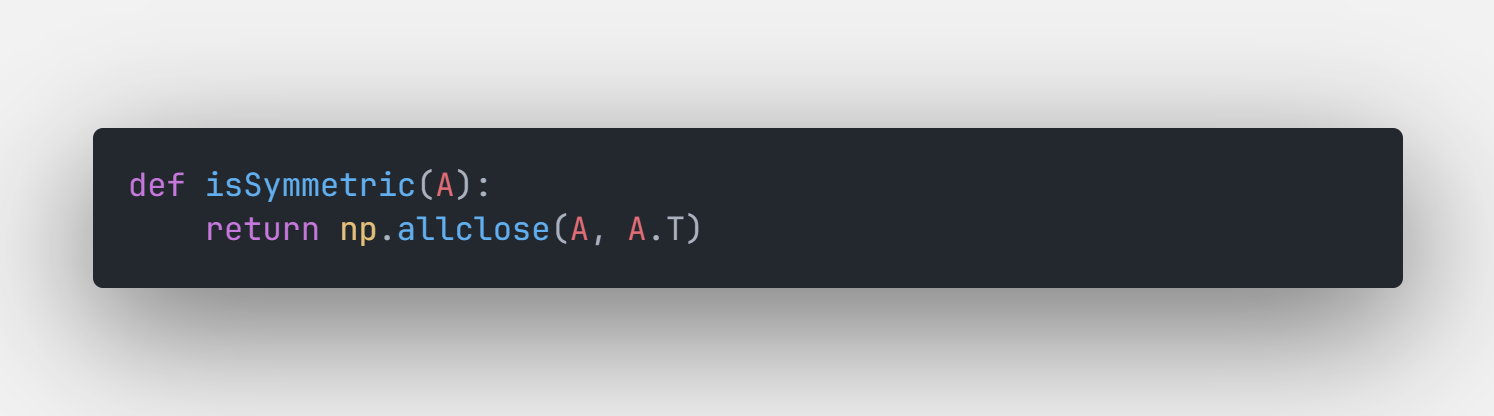
\includegraphics[width=1\textwidth]{isSymmetric.png}
      \caption{Función \texttt{isSymmetric}}
  \end{figure}

  al ejecutar esta función sobre nuestra matriz $A$, se obtiene que no es simétrica. Debido a esto, no se cumple el primer supuesto requerido para aplicar los métodos de Gradiente Descendiente y Gradiente Conjugado y por ende no podemos aplicarlos a nuestro problema.

  \paragraph{}
  Una vez cubiertos los métodos y sus supuestos, procederemos a compararlos bajo el número de iteraciones que necesitaron para alcanzar una tolerancia de $1\times10^{-6}$. A continuación los parámetros y soluciones:

  \[N_x=60, \ N_y=20, \ V_x^0=1, \ V_y^0=0.001, \ h=0.001\]

  \begin{figure}[H]
      \centering
      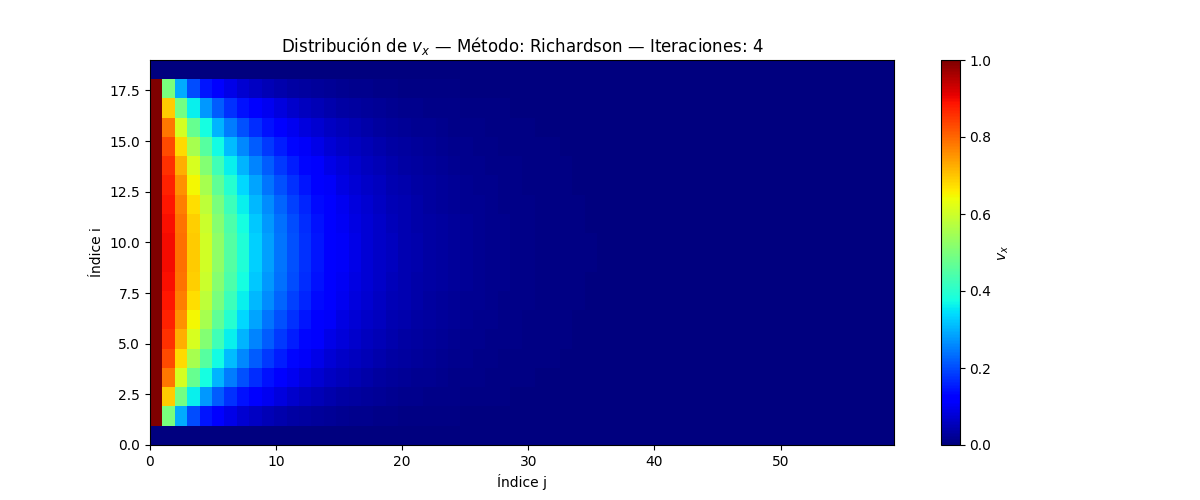
\includegraphics[width=1.2\textwidth]{Richardson.png}
      \caption{Solución mediante Richardson}
  \end{figure}

  \begin{figure}[H]
      \centering
      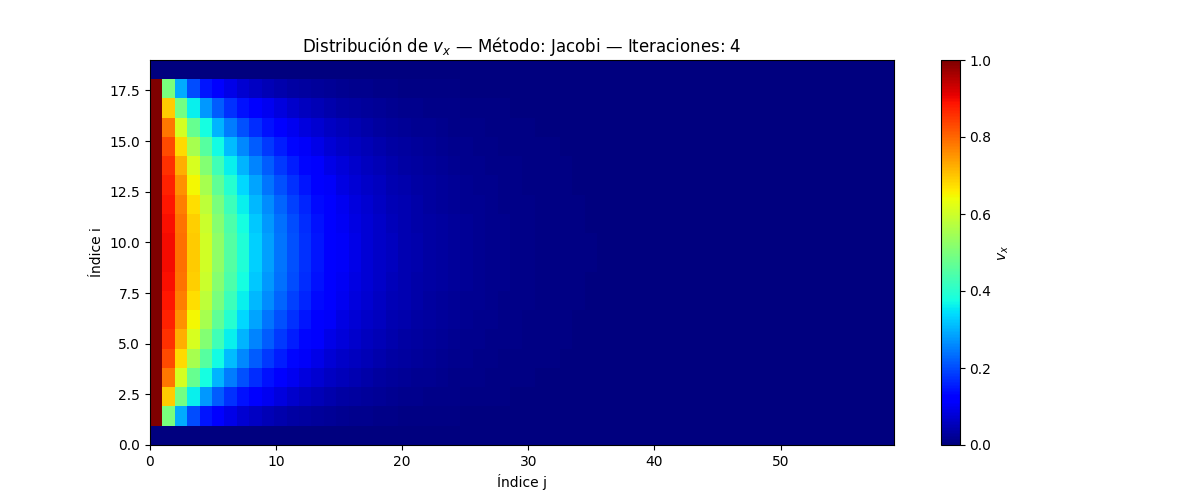
\includegraphics[width=1.2\textwidth]{Jacobi.png}
      \caption{Solución mediante Jacobi}
  \end{figure}

  \begin{figure}[H]
      \centering
      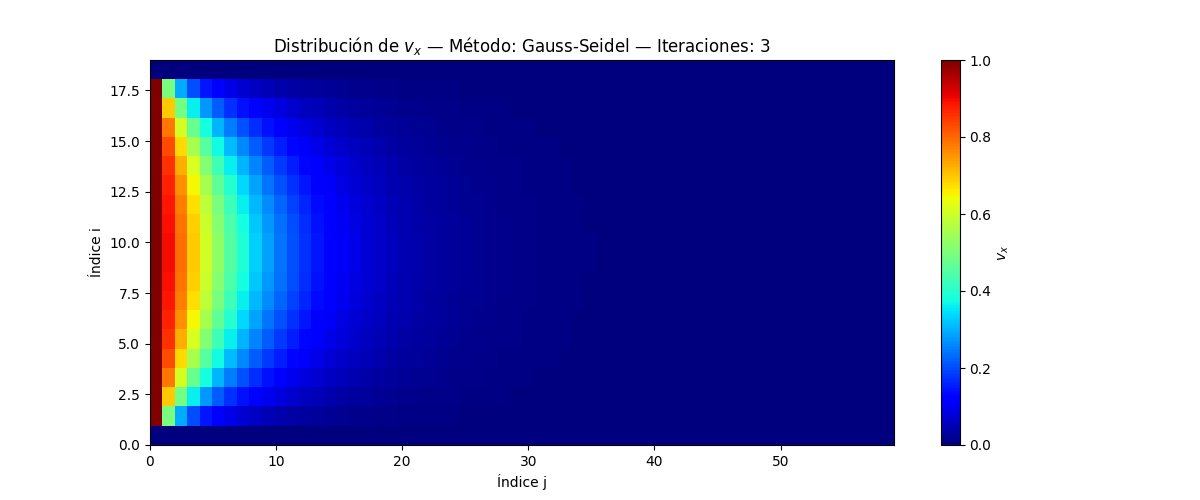
\includegraphics[width=1.2\textwidth]{GaussSeidel.png}
      \caption{Solución mediante Gauss Seidel}
  \end{figure}

  \section*{Conclusiones}

  \renewcommand{\refname}{Referencias}
  \bibliographystyle{plain}
  \bibliography{referencias}

\end{document}